\section{Komponenten die Gesamtanwendung}
\setauthor{Hain Lukas}

\begin{figure}[H]
    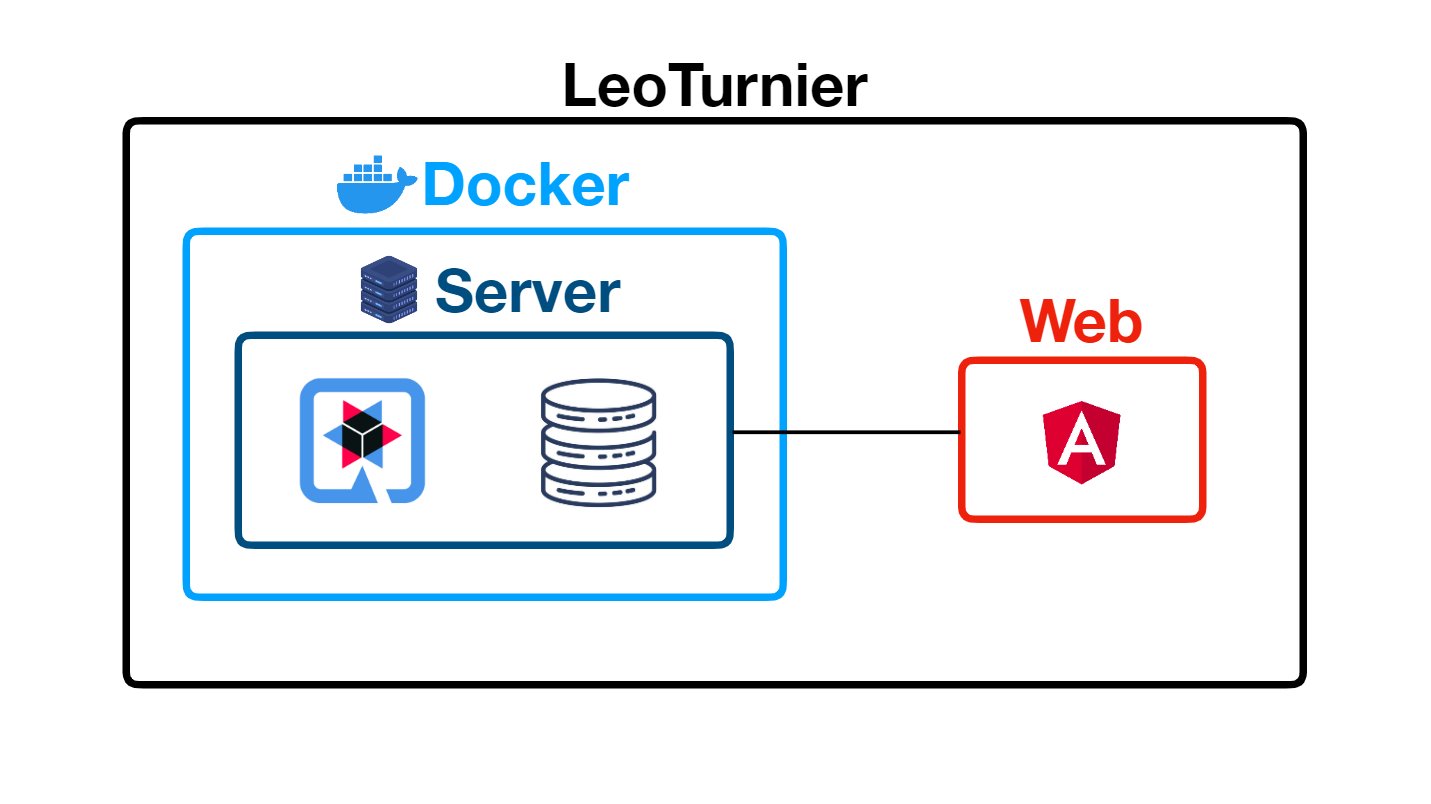
\includegraphics[scale=0.30]{pics/system_architecture.png}
    \caption{system architecture}
\end{figure}

Die Diplomarbeit ist Aufgeteilt in Frontend und Backend. 

\subsection{Backend}
\setauthor{Hain Lukas}

Im Backend befindet sich eine Quarkus Applikation. Sie wurde in Java geschrieben und verwaltet mithilfe von "Hibernate ORM with Panache" Turnierdaten in einer PostgreSQL Datenbank.
Diese Daten werden dem Frontend mithilfe von "RESTEasy" zur Verfügung gestellt. Außerdem befindet sich im Backend ein KeyCloak Server, der Userdaten in einer weiteren PostgreSQL Datenbank 
verwaltet. Die Quarkus Applikation, der KeyCloak Server und die beiden PostgreSQL Datenbanken werden in jeweils einem Docker Container ausgeführt.

\subsection{Frontend}
\setauthor{Ecker Benjamin}

TODO

\section{Verwirklichung der Anforderungen}

TODO